\documentclass[12pt,a4paper]{extarticle}

\usepackage{extsizes}	
\usepackage[english,russian]{babel}
\usepackage[utf8]{inputenc}
\usepackage{verbatim}
\usepackage{algorithm}
\usepackage{clrscode}
\usepackage{varwidth}
\usepackage{xcolor}
\usepackage[final]{graphicx}
\usepackage{amsmath, amssymb}
\usepackage{amsthm}
\usepackage[left=30mm,right=15mm,top=20mm,bottom=25mm]{geometry}
\usepackage{setspace}
\onehalfspacing 

\setcounter{page}{2}

\usepackage{pictures_examples}

\usepackage[final]{graphicx}
\usepackage{pstricks-add,pst-node,pst-text,pst-3d}
\usepackage{pgf, pgfarrows,pgfnodes,pgfautomata,pgfheaps,pgfshade}
\usepackage{tikz}
\usepackage{amsmath, amssymb}
\usepackage{amsthm}
\usepackage{pictures}

%%abbreviations
\newcommand{\mbabbr}[0]{МБ}
\newcommand{\mlnabbr}[0]{млн}
\newcommand{\secabbr}[0]{сек}
\newcommand{\minabbr}[0]{мин}

\newtheoremstyle{break}% name
  {9pt}%      Space above, empty = `usual value'
  {9pt}%      Space below
  {\itshape}% Body font
  {}%         Indent amount (empty = no indent, \parindent = para indent)
  {\bfseries}% Thm head font
  {.}%        Punctuation after thm head
  {\newline}% Space after thm head: \newline = linebreak
  {}%         Thm head spec

\theoremstyle{break}
\newtheorem{theorem}{Теорема}
\newtheorem{lemma}{Лемма}
\newtheorem{example}{Пример}

\bibliographystyle{unsrt} 
\begin{document}

\tableofcontents

\newpage
\section{Введение}
С каждым годом растет объем доступных данных. Как следствие, все чаще возникает
задача по обработке большого объема данных. Классические строковые алгоритмы
напрямую зависят от размера входных данных. Более того, начиная с некоторого
размера входа они просто не применимы для решения задач, так как ориентированы в
основном на работу в оперативной памяти. Для того, чтобы справиться с растущим
объемом входных данных, возникают новые классы алгоритмов, которые принципиально
отличаются от классических строковых алгоритмов. Так, например, есть класс
алгоритмов, которые хранят и обрабатывают входные данные с помощью файловой
системы. Минусом этих алгоритмов является то, что  они существенно медленней,
чем классические, однако позволяют обработать несравнимо больший объем данных.
Другим классом алгоритмов является класс алгоритмов обработки сжатых
представлений.

Грамматическое сжатие является одним из применяемых методов сжатия данных.
Его основной принцип -- построение по строке некоторой грамматики, из которой эта строка
выводится единственным образом.

Главным преимуществом грамматического сжатия является то, что оно позволяет
производить операции со сжатой строкой без предварительной распаковки. Примером
такой операции может служить использование строки в сжатом виде во время поиска
подстроки в строке.

Грамматическое сжатие может быть применено в биологии для хранения
\\ДНК-последовательностей. ДНК-последовательности занимают большие объемы,
поэтому обычно они хранятся в сжатом виде. Возможность работать со строкой, не
разжимая ее, является преимуществом грамматического сжатия. Примером
использования такого представления может служить извлечение информации об
образцах в исходной строке, а конкретно, грамматическое сжатие используется для
распознавания образцов в ДНК-последовательностях~\cite{appr_alg}.

Грамматическое сжатие хорошо работает и в случаях, когда строка представляет из
себя одно слово, тогда как традиционные методы поиска в больших объемах данных
подразумевают, что текст разбит на слова (например, построение обратного
индекса).

Задача построения минимальной грамматики является $NP$-трудной~\cite{np},
поэтому существенный интерес представляют эвристики. В данной
работе предложен алгоритм приближенного построения прямолинейных программ,
который ориентирован на параллельное построение.

\newpage
\section{Условные обозначения}
В данной работе рассматриваются строки над конечным алфавитом $\Sigma$.
Длина строки $S \in \Sigma^*$ равна количеству символов из $\Sigma$ в $S$ и
будет обозначаться как $|S|$.
Позицией в строке $S$ называется место между соседними символами.
Позиция 0 предшествует строке $S$, а позиция $|S|$ следует за строкой $S$. Для строки $S$
и числа $i$ такого, что $0 \leq i < |S|$, через символ $S[i]$ обозначается
символ, расположенный между позициями $i$ и $i+1$. Через $S[l\ldots r]$, где $0
\leq l < r \leq |S| - 1$, обозначается подстрока строки $S$, начинающаяся в
позиции $l$ и заканчивающаяся в позиции $r$. 

В качестве представления строки $S$ будут использоваться
контекстно-свободные грамматики. Контекстно-свободная грамматика
(КС-грамматика) -- это четверка вида $G = (\Sigma, \Gamma, P, S)$, где 
\begin{itemize}
\item $\Sigma$ -- конечный терминальный алфавит;
\item $\Gamma$ -- конечный нетерминальный алфавит ($\Sigma \bigcap \Gamma =
\oslash$);
\item $P$ -- множество правил вывода вида $A \rightarrow \alpha,\ A \in \Gamma,
\ \alpha \in (\Sigma \bigcup \Gamma)^*$;
\item $S \in \Gamma$ -- начальный символ (аксиома).
\end{itemize}

Прямолинейная программа (кратко ПП) -- это последовательность правил вывода
вида:

$X_1 = expr_1; X_2 = expr_2; \ldots; X_m = expr_m$,
где $X_i$ -- нетерминальный символ, а $expr_i$ -- это:
\begin{itemize}
\item $expr_i$ -- символ из алфавита $\Sigma$ (терминал), или
\item $expr_i = X_l \cdot X_r\ (l, r < i)$, где <<$\cdot$>> -- конкатенация
правил $X_l$ и $X_r$.
\end{itemize}

ПП является грамматикой в нормальной форме Хомского, выводящая единственную
строку.

\begin{example}
ПП, выводящая строку ``aaaababaabaaaabab'':
	\begin{center} 
		$X_1\ =\ a;\ X_2\ =\ b;\ X_3\ =\ X_1\cdot X_1;\ X_4\ =\ X_3\cdot X_3;$
		\\
		$X_5\ = X_1\cdot X_2;\ X_6\ =\ X_2\cdot X_5;\ X_7\ =\ X_4\cdot X_6;$
		\\
		$X_8\ = X_2\cdot X_1;\ X_9\ =\ X_3\cdot X_8;\ X_{10}\ =\ X_7\cdot X_9;$
		\\
		$X_{11}\ = X_1\cdot X_3;\ X_{12}\ =\ X_{11}\cdot X_6;\ X_{13}\ =\ X_{10}\cdot
		X_{12};$
	\end{center}
\end{example}

Каждой ПП можно сопоставить дерево вывода -- некоторое
упорядоченное корневое дерево, вершины которого помечены символами из $\Sigma
\bigcup \Gamma$. 

На рисунке~\ref{word_slp} представлено дерево вывода ПП, выводящей строку ``$aaaababaabaaaabab$''.

\begin{figure}
    \begin{center}
        \begin{picture}(85,105)(120,10)
            \picExample{}
        \end{picture}
    \end{center}
    \caption{ПП, выводящая строку ``$aaaababaabaaaabab$''}
    \label{word_slp}
\end{figure}

Для представления дерева вывода ПП будет использоваться $AVL$-дерево.
$AVL$-дерево – это двоичное дерево, у каждого внутреннего узла которого высоты
сыновей отличаются не более чем на 1.

$AVL$-грамматиками называются ПП, деревья вывода которых являются $AVL$-деревьями. 

Пусть $A \in \Gamma$. Тогда $val(A)$ -- строка из терминалов, выводимая из $A$.

\newpage
\section{Постановка задачи}
Задачу построения ПП можно сформулировать следующим
образом:

Вход: Строка $S \in \Sigma^*$.

Выход: ПП, выводящая $S$.

Критерий оценивания: Размер получившейся ПП и скорость её построения.   

Известно, что задача построения грамматики минимального размера для
заданной строки является $NP$-трудной ~\cite{np}. Поэтому для построения ПП
используются эффективные приближенные алгоритмы. В данной работе для построения ПП будет
использоваться подход, предложенный Риттером~\cite{rytter}. Этот подход
предполагает представление строки в виде $LZ$-факторизации. 

$LZ$-факторизацией строки $S$ ($LZ(S)$) называется представление $S$ как 
$f_1 \cdot f_2 \cdot \ldots \cdot f_k$, где $f_1 = S[1]$, и для любого $1 < l
\leq k, f_l$ - это наибольший префикс $f_l \cdot \ldots \cdot f_k$, который
встречается в $f_1 \cdot \ldots \cdot f_{l-1}$. Каждый $f_l$ называется
фактором. Размером $|LZ(S)|$ называется количество факторов в $LZ(S)$.

Исходя из этого, можно переформулировать исходную задачу в следующем виде: 

Вход: Строка $S$ и ее факторизация $LZ(S)$.

Выход: ПП, соответствующая $S$.

При использовании данного подхода для заданной строки $S$ можно построить ПП за
время $O(k\log n)$, размер которой будет $O(k\log n)$, где $n$ - длина $S$,
$k$ - размер $LZ(S)$~\cite{rytter}.

\newpage
\section{Обзор уже существующих алгоритмов построения ПП}
В рамках проблемы построения минимальной ПП проводились исследования, в ходе
которых были предложены алгоритмы приближенного решения данной проблемы. В
работе будет приведен обзор двух таких алгоритмов. 

\subsection{Алгоритм Риттера}
В 2003 году Риттером~\cite{rytter} был представлен алгоритм грамматического сжатия,
использующий представление строки в виде $LZ$-факторизации и
основывающийся на $AVL$-грамматике.

На вход алгоритму передается строка $S$, $|S| = n$. После чего происходит
вычисление $LZ$-факторизации $f_1 \cdot f_2 \cdot f_3 \cdot \ldots \cdot
f_k$ строки $S$, которая может быть вычислена за время $O(n\
log|\Sigma|)$, используя суффиксные деревья. Если $LZ$-факторизация достаточно
большая (превышает $n/log(n)$), тогда можно пренебречь алгоритмом и
сгенерировать тривиальную грамматику размера $n$, соответствующую данной строке.
Иначе происходит обработка $LZ$-факторизации слева-направо по следующему
алгоритму. 
Предположим, что для некоторого префикса $f_1 \cdot f_2 \cdot f_3  \cdot \ldots
 \cdot f_{i-1}$ уже построена ``хорошая'' ($AVL$-сбалансированная и размера $O(i\log n)$)
грамматика $G$. Если $f_i$ - терминальный символ, то генерируется подходящий
нетерминал $A$ и  $G := Concat(G, A)$. Иначе в префиксе $f_1 \cdot f_2 \cdot f_3 \ldots f_{i-1}$ ищется
сегмент, который соответствует $f_i$. Используя тот факт, что $G$ сбалансированная, можно найти
логарифмическое число нетерминалов $S_1, S_2, \ldots, S_{t(i)}$ из $G$, таких
что $f_i = val(S_1) \cdot val(S_2) \cdot \ldots val(S_{t(i)})$.
Последовательность $S_1, S_2, \ldots, S_{t(i)}$ назовем грамматическим
представлением фактора $f_i$.

После этого производится конкатенация частей грамматики, соответствующих
нетерминалам $G$, используя операцию $Concat$. Можно
заметить, что первые $|\Sigma|$ нетерминалов соответствуют буквам алфавита,
которые встретились в начале. Инициализация $G$ производится  первым символом $S$ и содержит все
нетерминалы для терминальных символов. 

На рисунке~\ref{rytter} представлен псевдокод описанного алгоритма.

Немного подробнее остановимся на операции конкатенации двух грамматик
$Concat(A, B)$. Для этого рассмотрим операцию конкатенации двух деревьев вывода
этих грамматик, $T1$ и $T2$ соответственно. Каждое из них является
$AVL$-деревом, но в данном случае случае каждое дерево грамматики содержит ключи
(символы) только в листьях, поэтому конкатенируя два дерева грамматик не нужно
удалять корень одного из них (это подразумевает дорогостоящую перестройку
дерева). Пусть $height(T1) \geq height(T2)$, другой случай является
симметричным. Идя по правой ветви $T1$ можно заметить, что высота узлов
уменьшается каждый раз не более чем на 2. Остановка происходит на 
некотором узле $v$ таком, что $height(v) - height(T2) \in$ \{1, 0\}.
Затем создается новый узел $v'$, отец которого является отцом $v$ и сыновья
которого $v$ и $root(T2)$. Получившееся дерево может быть несбалансированным по правой ветви.
В этом случае происходит перебалансировка получившегося $AVL$-дерева. 

\begin{figure}[!h]
	\begin{center}
	  \begin{varwidth}{\linewidth}
		\begin{codebox}
			\Procname{$\text{Алгоритм вычисления ПП}$}
				\li Вычисляем $LZ$-факторизацию $f_1f_2f_3 \ldots f_k$ 
				\li \If $k > n/\log(n)$
				\li 	\Then 
				\li			\Return тривиальная грамматика размера $O(n)$;
				\li \Else
				\li		\For $i = 1\ to\ k$ 
				\li			\Do
				\li		\textbf{(1)} Пусть $S_1, S_2, \ldots, S_{t(i)}$ -
				\\грамматическое представление $f_i$; 
				\li		\textbf{(2)} $H := Concat(S_1, S_2,
				\ldots, S_{t(i)})$; 
				\li		\textbf{(3)} $G := Concat(G,H)$;
				\End
				\End
				\li \Return $G$;
		\end{codebox}
		\caption{Псевдокод алгоритма Риттера}
		\label{rytter}
	  \end{varwidth}
	\end{center}
\end{figure}

\begin{example}
Рассмотрим пример работы данного алгоритма для строки ``aaaababaabaaaabab''.
$LZ$-факторизацией данной строки будет являться следующее представление:
\begin{center}
$f_1\ =\ a,\ f_2\ =\ a,\ f_3\ =\ aa,\ f_4\ =\ b,\ f_5\ =\ ab,\ f_6\ =\ aaba,\
f_7\ =\ aaabab$
\end{center}
Дерево вывода грамматики, построенное для данной строки, изображено на
рисунке~\ref{rytter_slp} (здесь приводится вариант без перебалансировок, чтобы
можно было видеть различия при сравнении с другими алгоритмами).

\begin{figure}[!h]
    \begin{center}
        \begin{picture}(85,160)(120,10)
            \picRytter{}
        \end{picture}
    \end{center}
    \caption{ПП, выводящая строку ``$aaaababaabaaaabab$''}
    \label{rytter_slp}
\end{figure}

\end{example}

\begin{theorem}
За время $O(n\log |\Sigma|)$ можно построить
приближение минимальному грамматическому сжатию с коэффициентом $O(\log n)$. 
Используя $LZ$-факторизация длины $k$, можно построить соответствующую
грамматику размера $O(k\log n)$ за время $O(k\log n)$~\cite{rytter}.
\end{theorem} 

Узким местом данного алгоритма является использование $AVL$-деревьев, а именно
работа с ними затрудняется поддержанием баланса. Если после добавления нового
правила в дерево оно перестает быть сбалансированным, то полученное дерево
приходится перебалансировать с помощью локального преобразования, называемого
вращением. Существует два типа вращений, каждое из которых может порождать до
трех новых узлов, а так же сделать до трех узлов неиспользуемыми.

\begin{lemma}
Пусть $A, B$ - два нетерминала $AVL$-сбалансированной
грамматики. Тогда за время \\$O(|height(A)-height(B)|)$ можно построить
$AVL$-сбалансированную грамматику $G = Concat(A,B)$, где $val(G) = val(A) \cdot
val(B)$, добавлением не более $O(|height(A)-height(B)|)$ нетерминалов~\cite{rytter}.
\end{lemma}

Из леммы можно видеть, что при конкатенации $AVL$-грамматик существенно разной
высоты появляется много новых правил, при добавлении которых может возникнуть
необходимость в большом числе вращений. При повторении основного цикла
достаточное число раз, высота текущей $AVL$-грамматики становится большой, а при
каждом последующем выполнении основного цикла с $G$ конкатенируется
$AVL$-грамматика относительно небольшой высоты.

Эта проблема была рассмотрена в~\cite{slp}, где был предложен вариант ее
решения.

\newpage
\subsection{Простой онлайн алгоритм грамматического сжатия}
Данный алгоритм рассматривается в рамках~\cite{lca}. Он не основывается на идее
использования представления строки в виде факторизации. Однако этот алгоритм
интересен тем, что представляет собой существенно новый подход к данной
проблеме.

Основываясь на идее $LCA$, производится замена пары $XY$,
встречающейся в данной строке, на новый символ $Z$ и генерируется правило $Z \rightarrow XY$, после
чего все вхождения пары $XY$ в строку заменяются на $Z$. Таким образом, целью этого
алгоритма является сведение к минимуму количества различных нетерминалов.
Замена осуществляется использованием одного из трех правил.

Повторение -- это строка $x^k$ для некоторого символа $x$ и целого $k \geq 2$.
повторение $S[i,j] = x^k$ называется максимальным, если $S[i-1] \neq x$ и
$S[j+1] \neq x$.

\textbf{Первое правило (повторяющаяся пара)}: Пусть данная строка $S$ содержит
максимальное повторение $S[i,j] = a^k$. Тогда генерируется новое правило $A
\rightarrow aa$, для соответствующего нетерминала $A$ и производится замена
$S[i,j] = A^{k/2}$, если $k$ -- четное, либо $S[i,j-1] = A^{(k-1)/2}$ для
$k$ нечетного. 

\textbf{Второе правило (минимальная пара)}: Введем общий порядок над $\Sigma
\bigcup \Gamma$, с помощью которого каждый символ может быть представлен целым
числом. Если данная строка содержит подстроку $A_iA_jA_k$, причем $j < i, k$,
тогда вхождение $A_j$ назовем минимальным. Второе правило заключается в замене
всех таких пар $A_jA_k$ в $A_iA_jA_k$ на соответствующий нетерминал.

Пусть $d$ -- положительное целое число и $k = \lceil log\ d\rceil$. Индексное
дерево $T_d$ -- это корневое, упорядоченное, полное бинарное дерево, чьи листья
помечены $1,\ldots2^k$. Высотой узла $v$ назовем количество ребер в
наидлиннейшем пути от $v$ до потомка $v$. Тогда высоту наименьшего общего
предка листьев листьев $i, j$ обозначим как $lca(i,j)$.

\textbf{Третье правило (максимальная пара)}: При фиксированном порядке
алфавита, если текущая строка содержит подстроку $A_iA_jA_kA_l$, такую, что
числа $i,j,k,l$ возрастают либо убывают и $lca(j,k) > lca(i,j),\ lca(k,l)$,
тогда вхождение средней пары $A_jA_k$ называется максимальным. По третьему
правилу такая пара заменяются на соответствующий нетерминал.

Пару, заменяемую по одному из вышеуказанных правил, назовем специальной.

Онлайн алгоритм облегченного грамматического сжатия использует $h$ очередей
$q_1, q_2, \ldots, q_h$, где $q_i$ представляет собой кольцевой буфер. Каждая
$q_i$ играет роль буфера хранения части строки $S$.
Число $h$ ограничено $O(log\ n)$~\cite{lca}. Для каждой очереди введем следующие
операции:
\begin{itemize}
\item $enque(q_i,x)$: добавить символ $x$ в хвост очереди $q_i$.
\item $deque(q_i)$: вернуть голову очереди $q_i$ и удалить ее.
\item $head(q_i)$: вернуть голову очереди $q_i$.
\item $len(q_i)$: вернуть длину очереди $q_i$.
\end{itemize}
Длину каждой очереди можно ограничить константой~\cite{lca}.

Для линейного времени сжатия будет использоваться обратный словарь $D^R(x,y)$,
возвращающий нетерминал $z$, такой, что $z \rightarrow xy \in D$. Если $z
\rightarrow xy \notin D$, тогда в $D^R(x,y)$ создается новое правило
$z \rightarrow xy$ и возвращается только что созданный нетерминал $z$.

Псевдокод алгоритма приведен на рисунке~\ref{onlinelca}. Помимо этого, так же
приведены функции $IsPair$ и $InsertSymbol$, необходимые в ходе работы
алгоритма.

\begin{figure}[!h]
	\begin{center}
	  \begin{varwidth}{\linewidth}
		\begin{codebox}
			\Procname{$\proc{IsPair}(s, i)$}
				\li \If $s[i, i+1]\ or\ s[i+2, i+3]$ -- повторяющаяся пара
				\li 	\Then \Return $true;$
				\End
				\li	\If $s[i+1, i+2]$ -- повторяющаяся пара
				\li		\Then \Return $false;$
				\End
				\li \If $s[i, i+1]$ -- минимальная или максимальная пара 
				\li 	\Then \Return $true;$
				\End
				\li \If $s[i+1, i+2]$ -- минимальная или максимальная пара 
				\li		\Then \Return $false;$
				\End
				\li		\Return $true;$
		\end{codebox}
		\caption{Псевдокод функции $IsPair$}
		\label{ispair}
	  \end{varwidth}
	\end{center}
\end{figure}		

На вход функции $IsPair$ передается некоторая последовательность символов $s$
и позиция, начиная с которой ищется заменяемая пара. Процедура выбирает одну из пар $s[i, i+1]$ или
$s[i+1, i+2]$, которая будет заменена в соответствии с вышеуказанными правилами, причем $s[i, i+1]$
выбирается если пара $s[i+1, i+2]$ не является специальной.

\begin{figure}[!h]
	\begin{center}
	  \begin{varwidth}{\linewidth}
		\begin{codebox}
			\Procname{$\proc{InsertSymbol}(q_i, x)$}
				\li $enque(q_i,x);$
				\li \If $len(q_i) \geq 5$
				\li 	\Then
				\li		\If $IsPair(q_i, 1) = true$
				\li 		\Then 
				\li			\Comment случай 1: $q_i[1,2]$ заменяемая пара
				\li			$deque(q_i);$
				\li			$y_1 = deque(q_i);$
				\li			$y_2 = head(q_i);$
				\li			$z := D^R(y_1,y_2), update D;$
				\li			$InsertSymbol(q_{i+1}, z);$
				\li		\Else 
				\li			\Comment случай 2: $q_i[2,3]$ заменяемая пара	
				\li			$deque(q_i);$
				\li			$y_1 = deque(q_i);$
				\li			$InsertSymbol(q_{i+1}, y_1);$
				\li			$y_2 = deque(q_i);$	
				\li			$y_2 = head(q_i);$
				\li			$z := D^R(y_2,y_3), update D;$	
				\li			$InsertSymbol(q_{i+1}, z);$
				\End
				\End 
		\end{codebox}
		\caption{Псевдокод функции $InsertSymbol$}
		\label{insertsymbol}
	  \end{varwidth}
	\end{center}
\end{figure}

Функция $InsertSymbol$, псевдокод которой приведен на
рисунке~\ref{insertsymbol}, определяет, какая пара будет заменена на данном
шаге.
Если длина переданной очереди $q_i$ больше 5, то определяется, какая именно пара
$q_i[1,2]$ либо $q_i[2,3]$ будет заменена. В случае $q_i[1,2]$ данная пара заменятся на
соответствующий нетерминал $z$, $q_i[0,1]$ извлекаются из очереди и $z$
помещается в $q_{i+1}$. В случае замены $q_i[2,3]$ на $z$, $q_i[0,2]$
извлекается и $q_i[1]z$ помещается в $q_{i+1}$. Символ $q_i[2]$ в первом случае
и $q_i[3]$ во втором запоминается в $q_j$ для определения следующей заменяемой
пары после добавления нового символа в $q_{i+1}$.

\begin{figure}[!h]
	\begin{center}
	  \begin{varwidth}{\linewidth}
		\begin{codebox}
			\Procname{$\proc{Online LCA}$}
				\li Создать пустые очереди $q_1,q_2, \ldots q_h;$
				\li $i := 1;$
				\li \While $i \leq h$
				\li		\Do
				\li 	$enque(q_i,d);$
				\li 	$i := i + 1;$
				\End 
				\li \Repeat
				\li		считать символ $c;$
				\li		$InsertSymbol(q_1,c);$
				\li \Until $c$ не является символом конца.
				\li Обработать символы, оставшиеся в очередях;
				\li \Return $D;$
		\end{codebox}
		\caption{Псевдокод функции $Online LCA$}
		\label{onlinelca}
	  \end{varwidth}
	\end{center}
\end{figure}

В начале работы алгоритма все очереди инициализируются фиктивным символом $d
\notin \Sigma \bigcup \Gamma$, который необходим для вычисления первой пары в
каждой очереди. В строках 7-10 алгоритма входные символы помещаются в очередь
$q_1$ друг за другом и вызывается функция $InsertSymbol$, которая рекурсивно
обрабатывает помещаемые символы. Алгоритм продолжает работу, пока все входные
символы не будут помещены в очередь. В конце происходит обработка символов,
оставшихся в очередях путем замены их на соответствующие нетерминалы в порядке
слева-направо. Результатом работы алгоритма является получившийся словарь
правил.

\begin{example}
Дерево вывода грамматики, построенное для строки ``aaaababaabaaaabab''  с
помощью данного алгоритма, изображено на рисунке~\ref{lca}. 
	\begin{figure}[!h]
	    \begin{center}
	        \begin{picture}(85,160)(120,10)
				\picLCA
			\end{picture}
	    \end{center}
	    \caption{ПП, выводящая строку ``$aaaababaabaaaabab$''}
	    \label{lca}
	\end{figure}
\end{example}

\begin{theorem} 
Время работы предложенного алгоритма можно оценить
$O(n)$, где $n$ - длина исходной строки~\cite{lca}.
\end{theorem}

\begin{theorem}
Приближенное оценка отношения $\frac{g}{g_m}$ для 
предложенного алгоритма $O(log^2\ n)$, где $g$ - размер получающейся
грамматики, $g_m$ - размер минимальной грамматики, $n$ - длина исходной строки
~\cite{lca}.
\end{theorem}

В данном алгоритме, в отличии от алгоритма, предложенного Риттером, дерево вывода
получающейся грамматики не является сбалансированным, из-за чего трудно
оценить его высоту. Из-за этого возникает трудность использования данного
алгоритма для дальнейшего применения к построенной грамматике алгоритмов поиска.

\newpage
\section{Алгоритм ленивого построения ПП}

\subsection{Идея}
Первоначальной идеей для данного алгоритма был анализ $LZ$-факторизации
текста с точки зрения использования символов. Под использованием в данном случае
понимается частота употребления каждого символа текста в факторах (сколько раз
конкретный символ используется при построении фактора). Для того, чтобы было
удобней воспринимать частоты с точки зрения факторизации без привязки к
конкретным символам, был осуществлен пересчет этих частот на факторы. В этом
случае, у каждого фактора из факторизации появляется вес, который определяется
отношением суммы соответствующих ему частот символов к длине подстроки,
соответствующей данному фактору.
Благодаря этому расширению понятия фактора, дальнейшую работу можно производить с точки
зрения фактора и его веса, абстрагируясь от частот конкретных символов строки.
Узнав вес каждого фактора, появилась возможность проанализировать частоту
использования каждого фактора. Для факторов с большим весом
количество использований подстроки, ему соответствующей, было большим, чем у фактора с
меньшим весом. Поэтому вполне естественным будет предположение о
порядке обработки каждого фактора. В алгоритме Риттера факторы обрабатывались
один за другим в соответствии с их порядком в $LZ$-факторизации. В данном случае
можно обрабатывать факторы в зависимости от их веса. Это позволит в начале
построить факторы, которым соответствуют самые часто используемые
подстроки, а значит когда будут строиться факторы с меньшим весом, то скорее
всего для подстроки, которой соответствует данный фактор, деревья вывода уже
будут построены и останется только сконкатенировать их. 

Далее будет рассмотрен алгоритм, основывающийся на предложенной идее.
Аналогично алгоритму Риттера, для построения ПП будут использоваться
$AVL$-грамматика.

\subsection{Структуры данных, которые понадобятся в ходе работы алгоритма}

Для эффективной работы алгоритма будут применены следующие структуры.

\begin{itemize}
\item Зависимости факторов \textbf{association(factor)}

Данная структура позволяет по конкретному символу узнать какой фактор ему
соответствует. Использование этой структуры позволяет найти декомпозицию
факторов, соответствующую данному. Ее можно мыслить как отображение \emph{$f_i
\rightarrow f_{i_1} \cdot f_{i_2} \cdot \ldots \cdot f_{i_l}$} и пару чисел,
указывающих где начало \emph{$f_i$} в \emph{$f_{i_1}$} и конец в \emph{$f_{i_l}$}. 

\item Отображение фактора в дерево \textbf{treesMap(factor)}

Отображение, которое по фактору возвращает дерево, соответствующее этому
фактору. 
\end{itemize}

\subsection{Функции, которые понадобятся при работе алгоритма}

\begin{itemize}
\item Функция веса фактора \textbf{weight(factor)}

Функция веса фактора вычисляется как отношение суммы частот всех символов,
которые соответствуют данному фактору в исходной строке, к длине подстроки,
соответствующей данному фактору. 

\item Нахождение последовательности поддеревьев, соответствующей
заданным началу и концу \textbf{split(tree, begin, end)}

Данная функция аналогична нахождению грамматического представления фактора в
алгоритме Риттера. Результатом работы данной функции будет являться
последовательность поддеревьев, соответствующих подстроке $S[begin\ldots end]$.
Функция $split$ выполняется за время, не превышающее $O(\log n)$.

\item Объединение последовательности поддеревьев \textbf{concat(\emph{$t_{1}$, $t_{2}$, \ldots $t_{k}$})} 

На вход данной функции подается последовательность
деревьев, на выходе - дерево, соответствующее объединению исходных деревьев в
первоначальном порядке. Так же аналогично алгоритму Риттера.

\item Создание дерева \textbf{CreateTree(factor)}

Данная функция вызывается для каждого фактора для создания дерева вывода,
соответствующего данному фактору. Псевдокод данной функции приведен
на рисунке~\ref{createtree}.

\item Поиск дерева \textbf{Search(factor)}

Эта функция используется в функции \textbf{CreateTree(factor)}, если для данного
фактора дерево еще не создано. Псевдокод данной функции приведен
на рисунке~\ref{search}.

\end{itemize}

\begin{lemma}
Для произвольного фактора $f$ строки $S$ процедура
$CreateTree(f)$ создает дерево, соответствующее этому фактору, за время
$O(k^2\log n)$, где $n$ - длина строки $S$, $k$ - размер $LZ(S)$.
\end{lemma} 

\textbf{Доказательство:}  Рассмотрим работу функции $CreateTree(f)$ для
некоторого фактора $f$.

В начале работы функции проверяется не было ли построено дерево для $f$ ранее.
Если дерево уже построено, а значит, содержится в $treesMap$, то оно
достается из $treesMap$ и является результатом работы. Данный шаг требует $O(1)$ операций.

В противном случае для построения дерева для фактора $f$ возможны два случая: 
\begin{itemize}
  \item $|f|$ = 1.\\
В этом случае фактор $f$ является терминальным и для $f$ создается дерево $t$
с единственным узлом, выводящее $f$, которое сохраняется в $treesMap(f)$.
После чего $t$ возвращается как результат работы. Этот случай требует так же $O(1)$ операций.
  \item $|f|$ > 1.\\
В этом случае дерево строится с помощью процедуры $Search(f)$. В начале, для
фактора $f$ строится декомпозиция $factors$, используя структуру $association$.
Такое представление является единственным по определению $LZ$-факторизации. Для
каждого фактора $f_l$ из декомпозиции $factors$ создается дерево $t_l$ с помощью
функции $CreateTree$. Если для некоторого $f_l$ дерева еще
построено не было, то он так же представляется в виде декомпозиции факторов
$factors_l$ и для каждого $f_{l_j}$ из декомпозиции строится дерево $t_{l_j}$. В
худшем случае на некотором шаге получается декомпозиция терминальных факторов,
для которых время построения дерева равно $O(1)$.
Количество факторов в декомпозиции $factors$ не более чем $|f|$, тогда, с точки
зрения исходной последовательности факторов в факторизации, для любого фактора
$f_i$, количество факторов в декомпозиции не более чем $i$. Пусть $h_{max} = max\{height(t_l)\}$,
$h_{min} = min\{height(t_l)\}$ и в исходной последовательности факторов $f =
f_i$, тогда для конкатенации всех деревьев $t_l$ необходимое количество операций
можно оценить, используя \textbf{Лемму 1}, как $i\ast(h_{max}-h_{min}) \leq
i\ast h_{max} \leq i\ast \log |f_i| = i\ast \log |f|$. В худшем случае $\log |f|$
оценивается $\log n$ и общее число операций, необходимое для построения дерева
$t$ для  фактора $f$, равно $O(\sum_{i=1}^k i\log n)$ или $O(k^2\log n)$. Дерево $t$ является
результатом работы функции $Search$, которое затем сохраняется в $treesMap(f)$ и
функция $CreateTree$ завершает работу, вернув $t$.
\end{itemize}
Таким образом, время работы функции $CreateTree$ равно $O(k^2\log n)$. 
$\Box$

\begin{figure}[!h]
	\begin{center}
	  \begin{varwidth}{\linewidth}
		\begin{codebox}
			\Procname{$\proc{CreateTree}(f)$}
				\li $Tree\ t = treesMap(f);$
				\li \If $t == null$ 
				\li		\Then
				\li		\If $f.isTerminal$ 
				\li			\Then 
				\li				$t = newTree(f.symbol);$
				\li			\Else 
				\li				$tree = Search(f);$ 
						\End
				\li				$treesMap(f) = tree;$	
					\End
				\li	\Return $tree;$
		\end{codebox}
		\caption{Псевдокод функции $CreateTree$}
		\label{createtree}
	  \end{varwidth}
	\end{center}
\end{figure}


\begin{figure}[!h]
	\begin{center}
	  \begin{varwidth}{\linewidth}
		\begin{codebox}
			\Procname{$\proc{Search}(f)$}
				\li	$factors = association(f);$
				\li	$trees = \{\};$
				\li	\For $Factor factor : factors$
				\li		\Do
				\li		$trees.add(createTree(factor));$
						\End
				\li	$Tree\ firstTree = trees.item(0);$
				\li \If $firstTree.absoluteBeginPosition \neq f.begin$
				\li		\Then 
				\li		$trees.delete(0);$
				\li		$trees.addToHead(split(firstTree, f.begin, firstTree.end));$
					\End
				\li	$Tree\ lastTree = trees.item(trees.length - 1);$
				\li \If $lastTree.absoluteEndPosition \neq f.end$
				\li 	\Then 
				\li		$trees.delete(trees.length - 1);$
				\li		$trees.add(split(lastTree, lastTree.begin, f.end));$
				 	\End
				\li	$tree = concat(trees);$ 	
				\li \Return $tree;$
		\end{codebox}
		\caption{Псевдокод функции $Search$}
		\label{search}
	  \end{varwidth}
	\end{center}
\end{figure}


\newpage
\subsection{Алгоритм}

\begin{enumerate}
  \item На вход алгоритму подается уже построенная факторизация
  $factorization$ строки $S$. По ней вычисляются частоты использования символов в факторизации. 
  \item Для каждого фактора \emph{$f_{i}$} из факторизации  вычисляется его вес
  \emph{$w_{i}$} = $weight$.
  \item Все факторы сортируются в зависимости от веса для получения новой
  последовательности \emph{$f_{j_1}$, $f_{j_2}$, \ldots
  $f_{j_k}$}.
  \item Для каждого фактора в новой последовательности строится соответствующее
  ему дерево
  \\$for\ (f : f_{j_1}, f_{j_2}, \ldots f_{j_k})$
  	\{\ $createTree(f);$\ \}
  \item В соответствии с первоначальной последовательностью факторов в
  факторизации происходит объединение всех факторов в одно дерево 
  $concat(treesMap(factorization))$.
\end{enumerate}

\begin{example}
Рассмотрим пример работы данного алгоритма для строки ``aaaababaabaaaabab''.
$LZ$-факторизацией этой строки является следующее представление:
\begin{center}
$f_1\ =\ a,\ f_2\ =\ a,\ f_3\ =\ aa,\ f_4\ =\ b,\ f_5\ =\ ab,\ f_6\ =\ aaba,\
f_7\ =\ aaabab$
\end{center}
Для каждого фактора $f_i$ его вес равен:
\begin{center}
$weight(f_1)\ =\ 3,\ weight(f_2)\ =\ 2,\ weight(f_3)\ =\ 2.5,\ weight(f_4)\ =\
4,\ weight(f_5)\ =\ 1.5,\ weight(f_6)\ =\ 0,\ weight(f_7)\ =\ 0$
\end{center}
Тогда факторы будут обрабатываться в следующем порядке: $f_4,\ f_1,\
f_3,\ f_2,\ f_5,\ f_6,\ f_7$.

Дерево вывода грамматики, построенное для данной строки, изображено на
рисунке~\ref{lazycslp} (здесь так же приводится вариант без перебалансировок,
чтобы можно было видеть различия при сравнении с другими алгоритмами).

\begin{figure}[!h]
    \begin{center}
        \begin{picture}(85,160)(120,10)
            \picLazyClassic
        \end{picture}
    \end{center}
    \caption{ПП, выводящая строку ``$aaaababaabaaaabab$''}
    \label{lazycslp}
\end{figure}

\end{example}

\newpage 
\subsection{Анализ предложенного алгоритма}

\begin{theorem}
Время работы данного алгоритма $max\{O(n),\ O(k^3\log
n)\}$, где $k$ - размер $LZ$-факторизации исходной строки $S$, $n$ - длина строки $S$.
\end{theorem} 

\textbf{Доказательство:} Оценим каждый шаг работы предложенного алгоритма. 
\begin{enumerate}
  \item Время выполнения этого шага алгоритма оценивается $O(n)$, при реализации
  его следующим образом: рассматривать каждый фактор $f_i$ из факторизации и для
  каждого символа из подстроки, соответствующей этому фактору, увеличивать счетчик
  использования этого символа.
  \item Данный шаг так же оценивается $O(n)$ для каждого фактора вычислять вес
  по имеющимся частотам.
  \item Здесь предполагается сортировка факторов в зависимости от веса,
  которую можно выполнить за время $O(k\log k)$ в среднем.
  \item Исходя из \textbf{Леммы 2} данный шаг осуществим за время $O(k^3\log
  n)$.
  \item Объединение всех факторов в одно дерево в исходной последовательности
  может быть реализовано за время $O(k\log n)$.
\end{enumerate}

Таким образом, время работы предложенного алгоритма $max\{O(n),\ O(k^3\log
n)\}$.
$\Box$

\begin{theorem} 
Для $AVL$-сбалансированной грамматики $G$, соответствующей
строке $S$, $|S|\ =\ n$, высота дерева вывода, соответствующего данной
грамматике $G$, равна $O(log\ n)$~\cite{rytter}.
\end{theorem} 

\begin{theorem}
Предложенный алгоритм строит грамматику, высота дерева вывода
которой равна $O(log\ n)$, где $n$ - длина строки $S$.
\end{theorem} 

\textbf{Доказательство:} Так как в качестве грамматики использовалась
$AVL$-сбалансированная грамматика, то по Теореме 5, высота дерева вывода
такой грамматики равна $O(log\ n)$.
$\Box$

\begin{theorem}
Размер памяти, необходимой для работы данного алгоритма,
равен $O(n)$, где $S$ - исходная строка, $n$ - длина строки $S$.
\end{theorem} 

\textbf{Доказательство:} Рассмотрим структуры, используемые в данном алгоритме.

\begin{itemize}
  \item $association$ позволяет получить  декомпозицию заданного фактора. В качестве ее
реализации можно использовать массив, в котором индекс соответствует номеру
символа в исходной строке, а значением является указатель на фактор из
$LZ$-факторизации, которому соответствует подстрока, которой принадлежит символ
с данным индексом. Для хранения данной структуры нам необходимо $O(n)$ памяти.
\item $treesMap$ хранит для каждого фактора соответствующее ему дерево. Для хранения
данной структуры нам необходимо $O(k)$ памяти, где $k$ - размер
$LZ$-факторизации.
\item Для вычисления частот символов на первом шаге алгоритма необходимо для каждого
символа хранить счетчик, соответствующий использованию данного символа. Это
можно реализовать используя $O(n)$ памяти.
\end{itemize}

Таким образом, для работы данного алгоритма необходимо $O(n)$ памяти.
$\Box$

Можно заметить преимущество алгоритма Риттера перед предложенным алгоритмом.
Для этого рассмотрим два фактора $f_i$ и $f_j$. Пусть $f_i$ можно представить в
виде $f_i = f_{i_1} \cdot f_{i_2} \cdot f_{i_3} \cdot \ldots
\cdot f_{i_k}$, а $f_j$ в виде $f_j = f_{j_1} \cdot f_{i_2} \cdot f_{i_3} \cdot
\ldots \cdot f_{j_m}$. При построении дерева для фактора $f_i$ будет построено
дерево для $f_{i_2} \cdot f_{i_3}$, в то же время при построении фактора $f_j$
дерево для $f_{i_2} \cdot f_{i_3}$ будет построено вновь, так как информации о
том, что деревья факторов $f_{i_2}$ и $f_{i_3}$ были объединены. Это повторное
построение дерева может замедлить как скорость работы алгоритма, так и увеличить
количество правил строящейся грамматики. В противоположность этому работает алгоритм Риттера, так как в нем дерево
строится по ходу и информация о том, объединялись ли данные деревья хранится
непосредственно в самом дереве, то такой ситуации не возникает.

Для исправления этой ситуации рассмотрим следующее изменение.

\newpage 
\subsection{Эвристическое улучшение алгоритма}

Для того, чтобы избежать повторного объединения существующих деревьев, добавим
метод $Refresh$, который будет осуществлять обновление структуры $association$.
Псевдокод этого метода приведен на рисунке~\ref{refresh}.

\begin{figure}[!h]
	\begin{center}
	  \begin{varwidth}{\linewidth}
		\begin{codebox}
			\Procname{$\proc{Refresh}(f,\ beginRefreshPosition)$}
				\li \For $i = beginRefreshPosition\ to\ beginRefreshPosition + f.length$
				\li		\Do
				\li			$association(i) = f;$
				\End
		\end{codebox}
		\caption{Псевдокод функции $Refresh$}
		\label{refresh}
	  \end{varwidth}
	\end{center}
\end{figure}

Параметрами данной функции являются фактор $f$ и целое положительное число
$beginRefreshPosition$, означающее, что с данной позиции и до
$beginRefreshPosition + f.length$ $association$ будет возвращать фактор $f$.

Помимо этого, изменится функция $Search$. Изменения продемонстрированы на
рисунке~\ref{searchnew}.

\begin{figure}
	\begin{center}
	  \begin{varwidth}{\linewidth}
		\begin{codebox}
			\Procname{$\proc{Search}(f)$}
				\li	$factors = association(f);$
				\li	$trees = \{\};$
				\li	\For $Factor factor : factors$
				\li		\Do
				\li		$trees.add(createTree(factor));$
						\End
				\li	$Tree\ leftTree = trees.remove(0),$\\ $middleTree = emptyTree,\ rightTree =
				trees.remove(trees.length - 1);$ 
				\li	$middleTree = concat(trees);$
				\li \If $leftTree.absoluteBeginPosition == f.begin$
				\li		\Then 
				\li		$tree = concat(leftTree, middleTree);$
				\li		$fakeFactor =$ \\ 
					$new\ Factor(f.beginPosition, tree.width, factors.item(0).absoluteBeginPosition);$ 
				\li		\If $rightTree.absoluteEndPosition == f.end$ 
				\li			\Then
				\li			$tree = concat(tree, rightTree);$
				\li			$treesMap(fakeFactor) = tree;$
				\li			$refresh(fakeFactor, factors.item(0).absoluteBeginPosition);$
				\li			\Else
				\li			$treesMap(fakeFactor) = tree;$
				\li			$refresh(fakeFactor, factors.item(0).absoluteBeginPosition);$
				\li			$tree = concat(tree, split(rightTree, rightTree.begin, f.end));$
				\End
				\li	\Else
				\li		$tree = middleTree;$
				\li		$fakeFactor =$ \\ 
					$new\ Factor(f.beginPosition, tree.width, factors.item(1).absoluteBeginPosition);$
				\li		\If $rightTree.absoluteEndPosition == f.end$
				\li			\Then
				\li			$tree = concat(tree, rightTree);$
				\li			$treesMap(fakeFactor) = tree;$
				\li			$refresh(fakeFactor, factors.item(1).absoluteBeginPosition);$
				\li			$tree = concat(split(leftTree, f.begin, leftTree.end), tree);$
				\li			\Else
				\li			$treesMap(fakeFactor) = tree;$
				\li			$refresh(fakeFactor, factors.item(1).absoluteBeginPosition);$
				\li			$tree = concat(split(leftTree, f.begin, leftTree.end),$\\ $tree,
				split(rightTree, rightTree.begin, f.end));$
				\End	
				\End
				\li \Return $tree;$
		\end{codebox}
		\caption{Псевдокод функции $Search$}
		\label{searchnew}
	  \end{varwidth}
	\end{center}
\end{figure}

Как и в первоначальном варианте, на вход данной функции передается фактор $f$,
для которого следует построить дерево. Для него с помощью $association$
находится декомпозиция, после чего осуществляется создание фактора, который будет
передаваться на вход функции $Refresh$. Он формируется исходя из наибольшего
дерева, которое может быть построено из следующий деревьев: ``среднего''
($middleTree$) - это дерево является объединением всех деревьев, за исключением
первого ($leftTree$) и последнего ($rightTree$). Далее рассматриваются 4
возможных случая размещения фактора относительно его декомпозиции:

\begin{enumerate}
\item Разница между левыми границами первого фактора в декомпозиции и фактора
$f$ равна 0 и разница между правыми границами последнего фактора и фактора
$f$ также равна 0. В этом случае все деревья (первое, ``среднее'' и последнее)
объединяются в одно, которое будет результатом работы процедуры, а так же
создается новый фактор ($fakeFactor$), начало которого соответствует
$f.beginPosition$, длина соответствует ширине получившегося дерева, а
$absoluteBeginPosition$ - это $absoluteBeginPosition$ первого фактора
декомпозиции, после чего вызывается функция $Refresh(fakeFactor)$.
\item Разница между левыми границами первого фактора в декомпозиции и фактора
$f$ равна 0, при этом разница между правыми границами последнего фактора и
фактора $f$ отлична от 0. В этом случае сначала объединяются первое и
``среднее'' деревья, происходит создание нового фактора с параметрами: его
начало соответствует $f.beginPosition$, длина соответствует ширине получившегося
дерева, а $absoluteBeginPosition$ - это $absoluteBeginPosition$ первого фактора
декомпозиции. После чего вызывается функция $Refresh(fakeFactor)$. Результатом
работы функции является объединение полученного ранее дерева с
последовательностью деревьев, соответствующих поддеревьям, получаемых из
последнего дерева от его начала и до конца фактора $f$.
\item Разница между левыми границами первого фактора в декомпозиции и фактора
$f$ отлична от 0 и разница между правыми границами последнего фактора и фактора
$f$ равна 0. В этом случае сначала объединяются ``среднее'' и последнее деревья
и происходит создание нового фактора с параметрами: начало соответствует
$f.beginPosition$, длина соответствует ширине получившегося дерева, а
$absoluteBeginPosition$ - это $absoluteBeginPosition$ второго фактора
декомпозиции. После чего вызывается функция $Refresh(fakeFactor)$. Результатом
работы функции является объединение последовательности деревьев, соответствующих
поддеревьям первого фактора с позиции, соответствующей $f.beginPosition$, и
получившегося дерева.
\item Разница между левыми границами первого фактора в декомпозиции и фактора
$f$ отлична от 0, при этом разница между правыми границами последнего фактора и
фактора $f$ отлична от 0. В этом случае просходит создание нового фактора с
параметрами: начало соответствует $f.beginPosition$, длина соответствует ширине
среднего дерева, а $absoluteBeginPosition$ - это $absoluteBeginPosition$ второго
фактора декомпозиции. После чего происходит вызов функции $Refresh(fakeFactor)$.
Результатом работы данной функции является объединение последовательности
деревьев, соответствующих поддеревьям первого фактора с позиции, соответствующей
$f.beginPosition$ со ``средним'' деревом и последовательностью деревьев,
соответствующих поддеревьям, получаемых из последнего дерева от его начала и до
конца фактора $f$.
\end{enumerate}

Каждое из созданных в ходе данного алгоритма деревьев так же сохраняются в
$treesMap$. 

Это изменение помогает избежать недостатка, возникающего ранее, а именно
повторного объединения деревьев, так как когда будет происходит
обращение к $association$ далее, на месте факторов, чьи деревья уже
объединялись, будет стоять недавно созданный фактор, которому соответствует
дерево с ранее объединенными деревьями.

\begin{example}
Рассмотрим пример работы данного алгоритма для строки ``aaaababaabaaaabab''.
$LZ$-факторизацией этой строки является следующее представление:
\begin{center}
$f_1\ =\ a,\ f_2\ =\ a,\ f_3\ =\ aa,\ f_4\ =\ b,\ f_5\ =\ ab,\ f_6\ =\ aaba,\
f_7\ =\ aaabab$
\end{center}
Для каждого фактора $f_i$ его вес равен:
\begin{center}
$weight(f_1)\ =\ 3,\ weight(f_2)\ =\ 2,\ weight(f_3)\ =\ 2.5,\ weight(f_4)\ =\
4,\ weight(f_5)\ =\ 1.5,\ weight(f_6)\ =\ 0,\ weight(f_7)\ =\ 0$
\end{center}
Тогда факторы будут обрабатываться в следующем порядке: $f_4,\ f_1,\
f_3,\ f_2,\ f_5,\ f_6,\ f_7$.

Дерево вывода грамматики, построенное для данной строки, изображено на
рисунке~\ref{lazyhslp} (здесь так же приводится вариант без перебалансировок,
чтобы можно было видеть различия при сравнении с другими алгоритмами).
\end{example}

\begin{figure}[!h]
    \begin{center}
        \begin{picture}(85,160)(120,10)
            \picLazyHeuristic
        \end{picture}
    \end{center}
    \caption{ПП, выводящая строку ``$aaaababaabaaaabab$''}
    \label{lazyhslp}
\end{figure}

Так как приведенные выше изменения не никак не влияют на $LZ$-факторизацию
исходной строки и не увеличивают количество факторов в декомпозиции для
некоторого фактора, оценки алгоритма, доказанные выше, остаются верными и в данном случае.

\newpage 
\subsection{Практические результаты}
На рисунках~\ref{dna_rotations},~\ref{dna_compression_ratio} и~\ref{dna_time} 
представлены графики работы данного алгоритма на ДНК-последовательностях.

График~\ref{dna_rotations} отображает количество вращений $AVL$-деревьев при
построении грамматики. По оси $OX$ расположена информация о
размере сжимаемого файла в МБ, а по оси $OY$ - размер получающейся
грамматики в миллионах. Как видно по данному графику, по сравнению с
классическим алгоритмом Риттера, количество вращений как для ленивого алгоритма, так и для его эвристического улучшения, значительно меньше. Не смотря на это, он уступает
модифицированному алгоритму Риттера~\cite{slp}. 

\begin{figure}[!h]
    \center{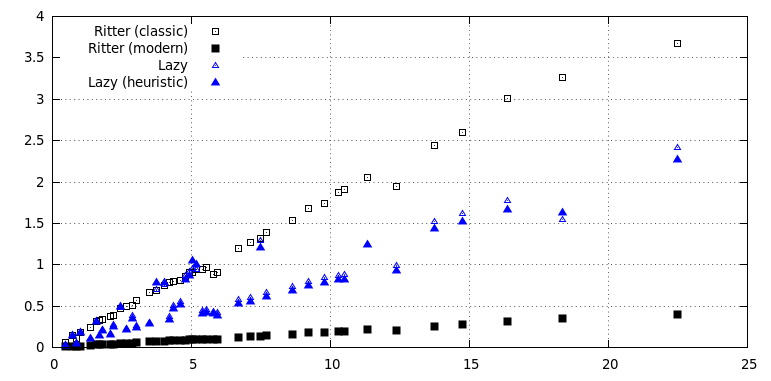
\includegraphics[width=1\linewidth]{images/Rebalances.png}}
    \caption{Вращения для ДНК}
    \label{dna_rotations}
\end{figure}

На графике~\ref{dna_compression_ratio} по оси $OX$ расположена информация о
размере сжимаемого файла в МБ, а по оси $OY$ указано отношение сжатого
представления к размеру исходного файла в процентах. Чем меньше это отношение,
тем лучше сжатие. Размер грамматики, получаемой с
помощью ленивых алгоритмов хуже, чем у алгоритма Риттера.

\begin{figure}[!h]
    \center{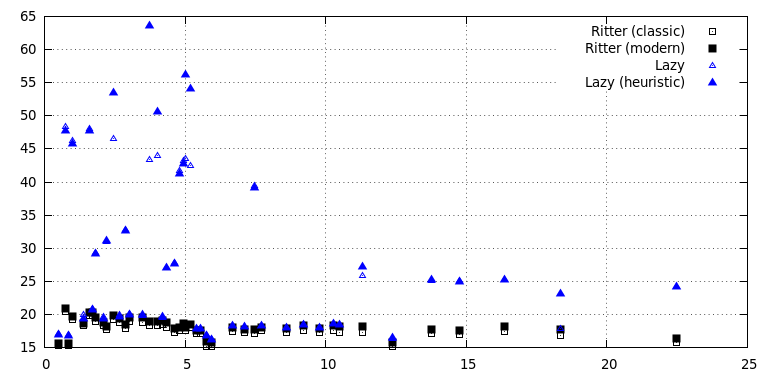
\includegraphics[width=1\linewidth]{images/Ratio.png}}
    \caption{Степень сжатия для ДНК}
    \label{dna_compression_ratio} 
\end{figure}

График~\ref{dna_time} отображает время работы алгоритмов. По оси $OX$
расположена информация о размере сжимаемого файла в МБ, а по оси $OY$ указано
время построения ПП в минутах. По нему можно судить, что скорость работы
ленивого алгоритма почти совпадает со скоростью работы его эвристического улучшения и лучше, чем скорость работы классического алгоритма
Риттера. Это позволяет судить о том, что доказанная оценка работы ленивого
алгоритма является оценкой худшего случая, так как на практике по полученным
данным можно судить, что существует более лучшая средняя оценка.

\begin{figure}[!h]
    \center{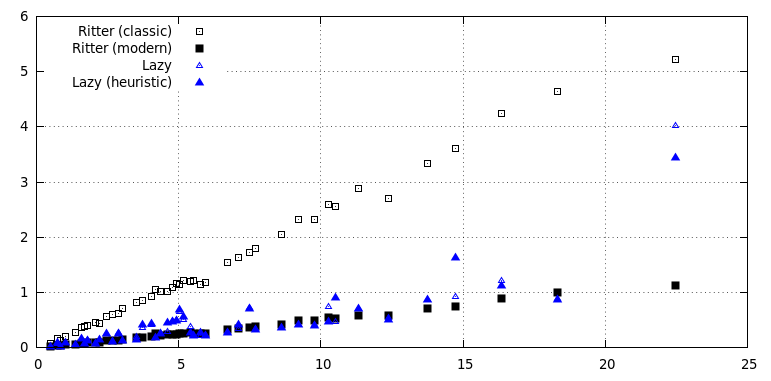
\includegraphics[width=1\linewidth]{images/Time.png}}
    \caption{Время построения для ДНК на файловой системе}
    \label{dna_time}
\end{figure}

Полученные практические результаты позволяют судить о том, что данный алгоритм
по некоторым параметрам лучше классического алгоритма Риттера. В частности можно
заметить, что предложенная эвристика работает не хуже, чем сам алгоритм, а
значит возможно дальнейшее развитие алгоритма с помощью улучшения этой эвристики.

\newpage 
\section{Выводы}

В данной работе предложен алгоритм построения прямолинейных программ. Было
предложено эвристическое улучшение данного алгоритма. Была доказана оценка его
работы в худшем случае. Был проведен практический сравнительный анализ с
алгоритмом Риттера.

Не смотря на то, что худшая оценка этого алгоритма $max\{O(k^3\log n), O(n)\}$,
на практике этот алгоритм показал себя лучше, чем классический алгоритм
Риттера.

Предложенный в данной работе алгоритм можно рассматривать как альтернативный
вариант алгоритма Риттера. По полученным практическим результатам видно, что
размер грамматики, построенный с помощью него, уступает размеру грамматики,
которая получается при использовании алгоритма Риттера. Однако характерной
особенностью здесь является подход к построению грамматики. В алгоритме Риттера
дерево грамматики строится за один проход и на каждом шаге построение некоторого
фактора напрямую зависит от уже построенного дерева. В то время как алгоритм,
предложенный в этой работе строит факторы таким образом, что не возникает
сильной зависимости от уже построенных факторов, так как каждый фактор строится
``по необходимости'', то есть лениво. Этот подход позволяет распараллелить
данный алгоритм. В данном случае участком распараллеливания будет является этап
построения деревьев для факторов, так как их построение слабо связано между
собой. Применение этого подхода позволит увеличить скорость работы алгоритма. В
противоположность этому, алгоритм Риттера распараллелить невозможно.



\newpage 

\begin{thebibliography}{5}

\bibitem{appr_alg} E. Lehman, A. Shelat, Approximation Algorithms for
Grammar-Based Compression, In Proceedings of the 13th ACM-SIAM Symposium on
Discrete Algorithms (2002), 205-212.
\bibitem{slp} I. Burmistrov, L. Khvorost, Straight-line programs: a practical
test, Proc. Int. Conf. Data Compression, Commun., Process., CCP (2011), 76–81.
\bibitem{np} M. Charikar, E. Lehman, D. Liu, R. Panigrahy, M. Prabhakaran, A.
Sahai, A. Shelat, The smallest grammar problem, IEEE Trans. Information Theory, 51 (2005), 2554–2576.
\bibitem{lca} S. Maruyama, M. Takeda, M. Nakahara, H. Sakamoto, An
Online Algorithm for Lightweight Grammar-Based Compression, First
International Conference on Data Compression, Communications and Processing
(2011).
\bibitem{rytter} W. Rytter, Application of Lempel-Ziv factorization to the
approximation of grammar-based compression, Theor. Comput. Sci., 302 (2003), 211–222.

\end{thebibliography}

\newpage
\thispagestyle{empty}
\begin{center}
	\textbf{РЕФЕРАТ}
\end{center}

Козлова А. В. Ленивое построение прямолинейных программ квалификационная работа
на степень бакалавра наук: 28 страниц, 16 рисунков, 5 источников.

Ключевые слова: прямолинейная программа, грамматическое сжатие, ленивое
построение.

Целью проделанной работы была разработка нового алгоритма построения
прямолинейных программ. В результате был разработан алгоритм, доказана оценка
его работы в худшем случае, предложена эвристика по улучшению этого алгоритма.
Так же было проведено сравнение этого алгоритма с алгоритмом Риттера на
практике.

\end{document}